\section{Принципы использования программного комплекса SearchInform для
мониторинга  утечек конфиденциальной информации}

\subsection{Ход работы}

\subsubsection{Определение списка пользователей, данные которых будут
перехватываться системой}

Запустим SearchInform NetworkSniffer Administrator Console и настроим
фильтр перехвата так, что после редактирования будут перехватываться данные
пользователей ivanov и bublik для всех контролируемых протоколов.
Результат настройки см. рис. \ref{fig:nsFilter}.

\begin{figure}[H]
  \centering
  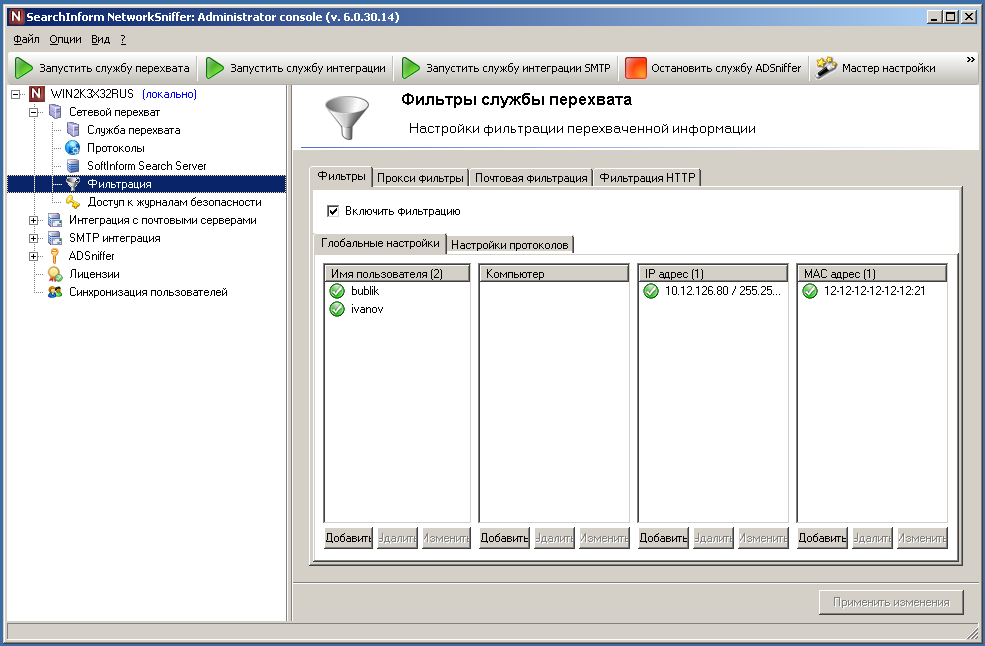
\includegraphics[width=\textwidth]{nsFilter}
  \caption{Результат настройки NetworkSniffer.}\label{fig:nsFilter}
\end{figure}

Скриншоты хода работы:

\begin{figure}[H]
  \centering
  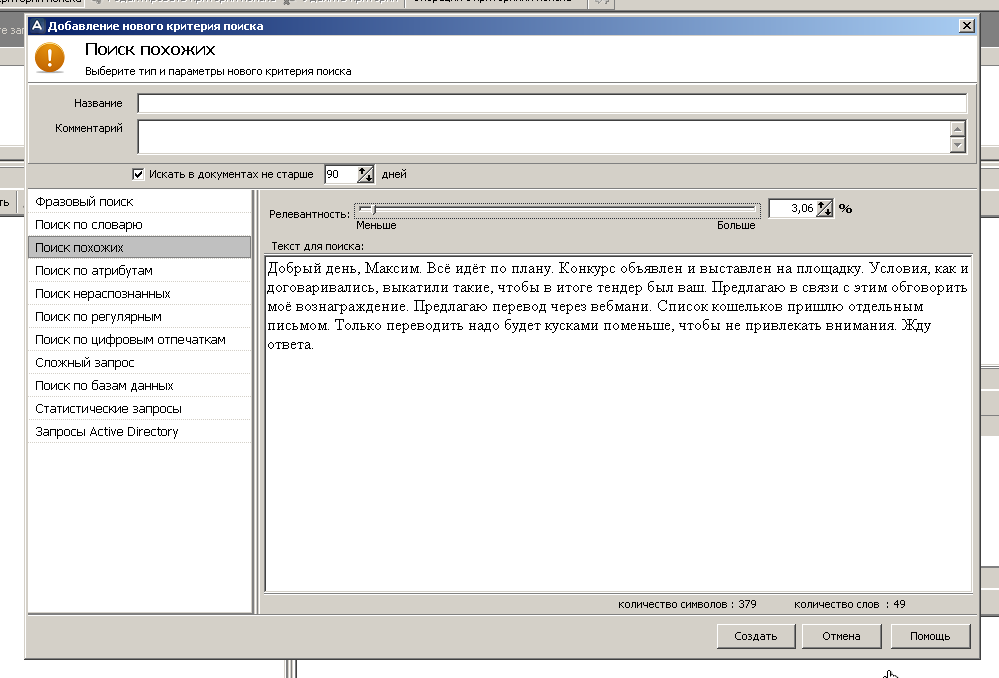
\includegraphics[width=\textwidth]{part2/1}
\end{figure}

\begin{figure}[H]
  \centering
  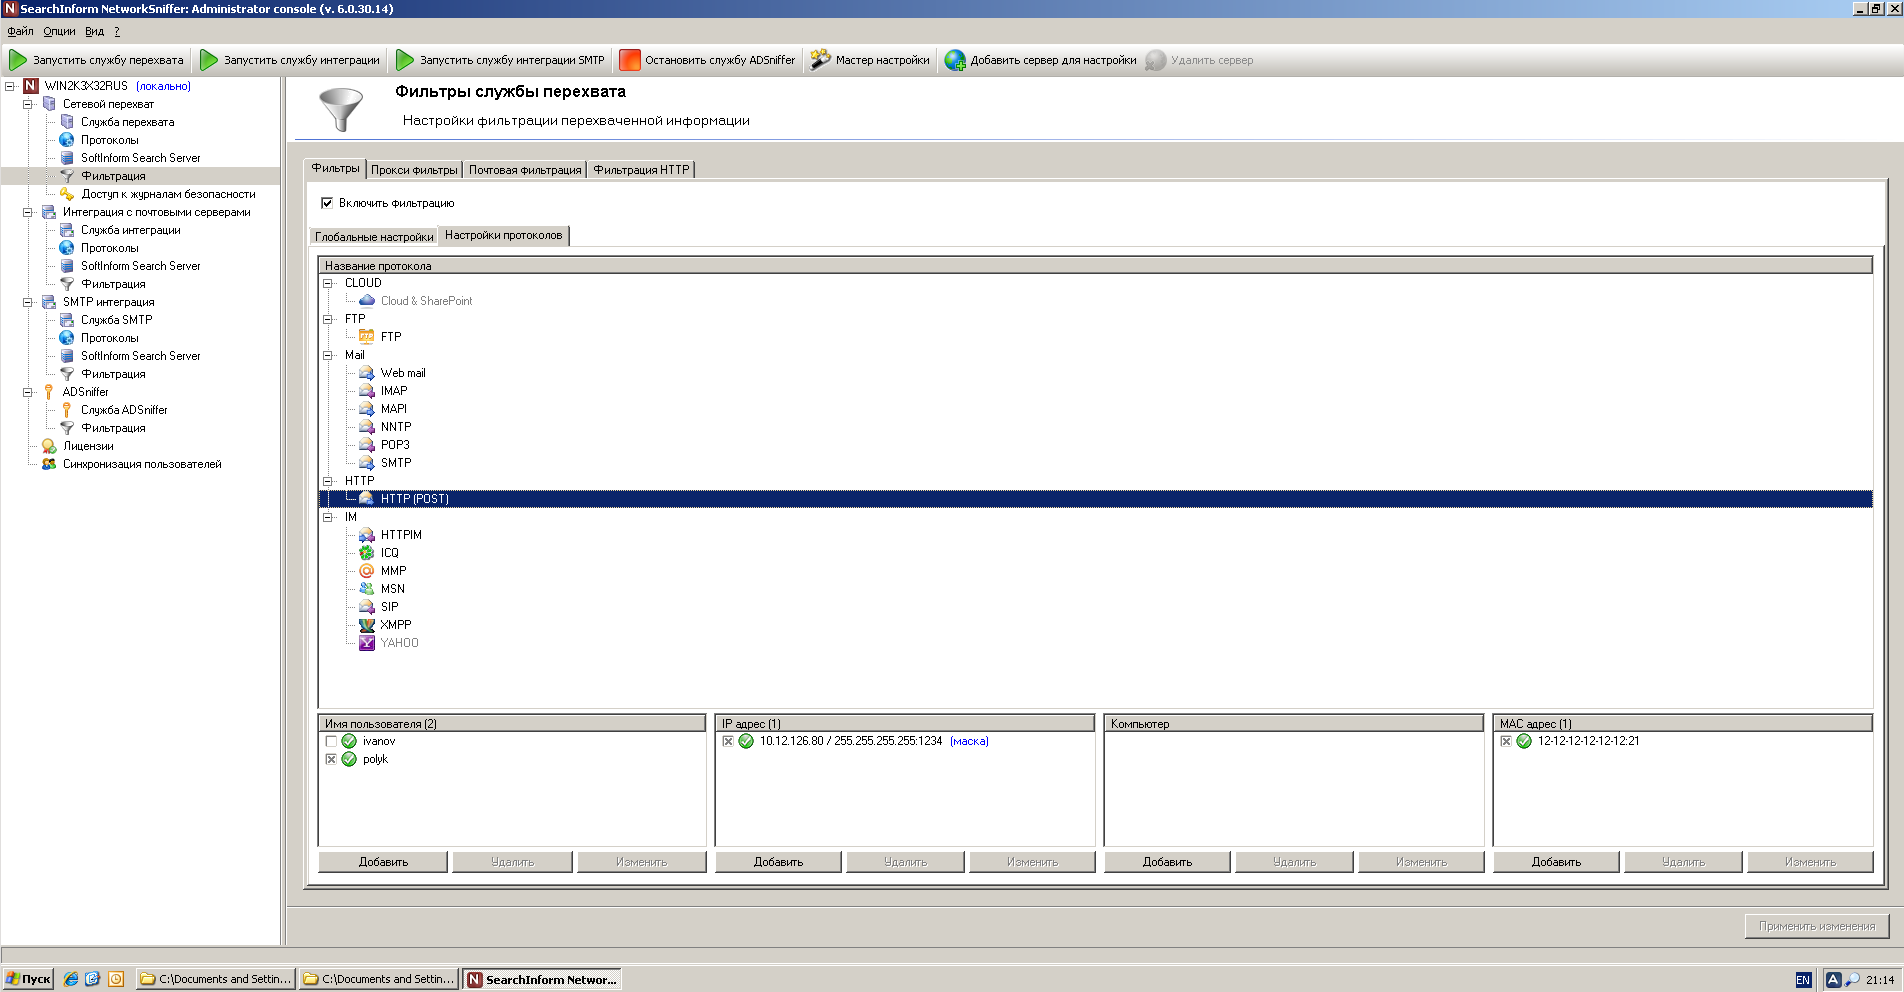
\includegraphics[width=\textwidth]{part2/2}
\end{figure}

\begin{figure}[H]
  \centering
  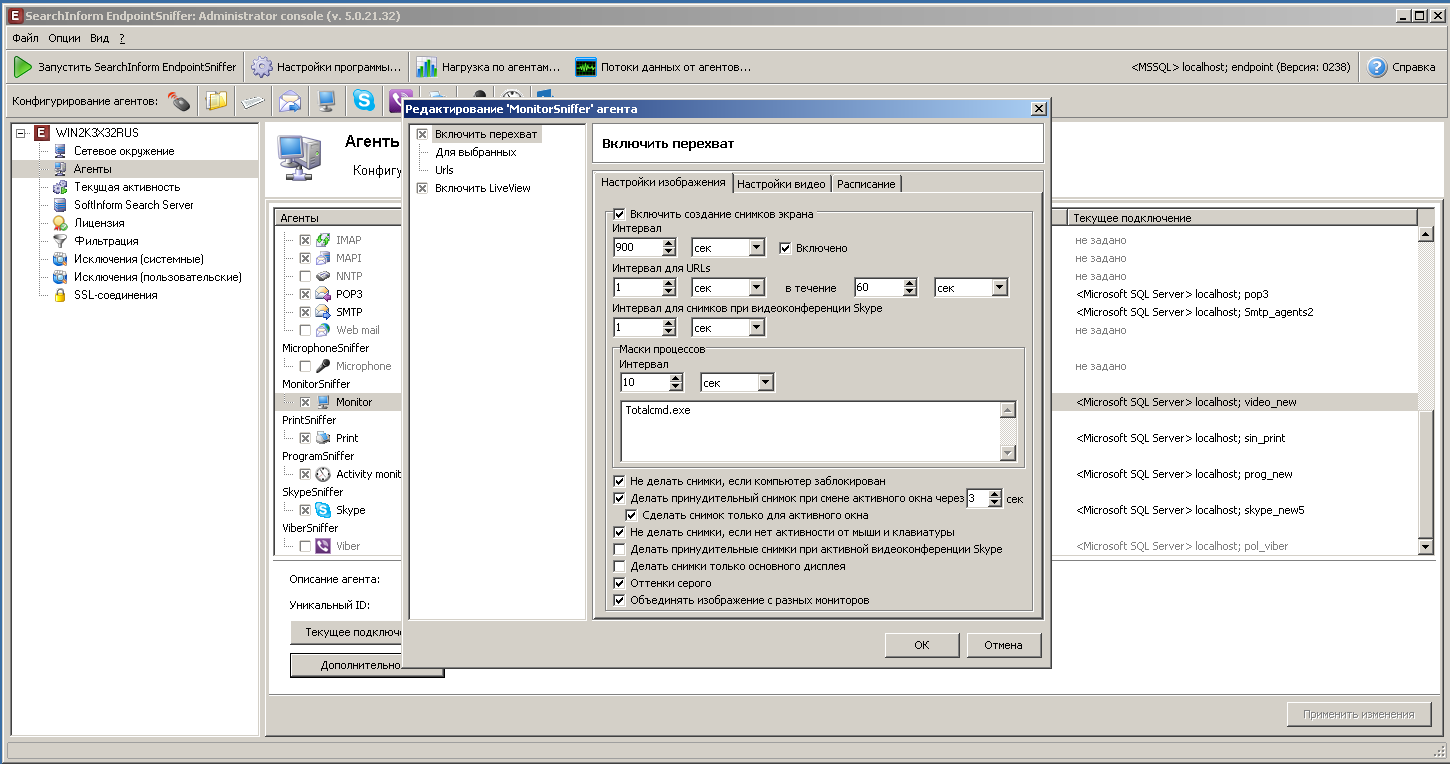
\includegraphics[width=\textwidth]{part2/3}
\end{figure}

\begin{figure}[H]
  \centering
  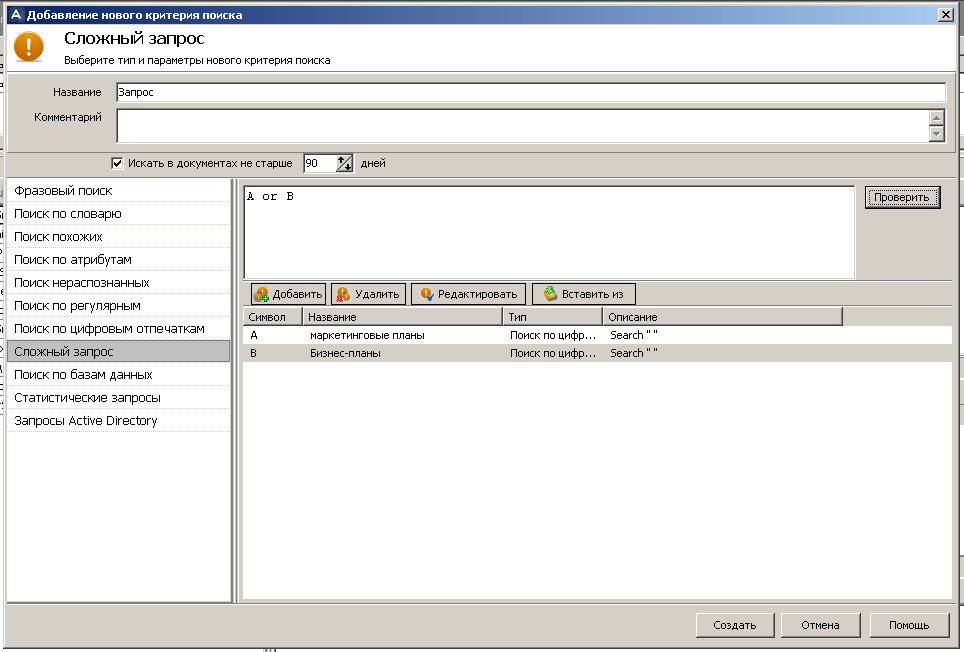
\includegraphics[width=\textwidth]{part2/4}
\end{figure}

\begin{figure}[H]
  \centering
  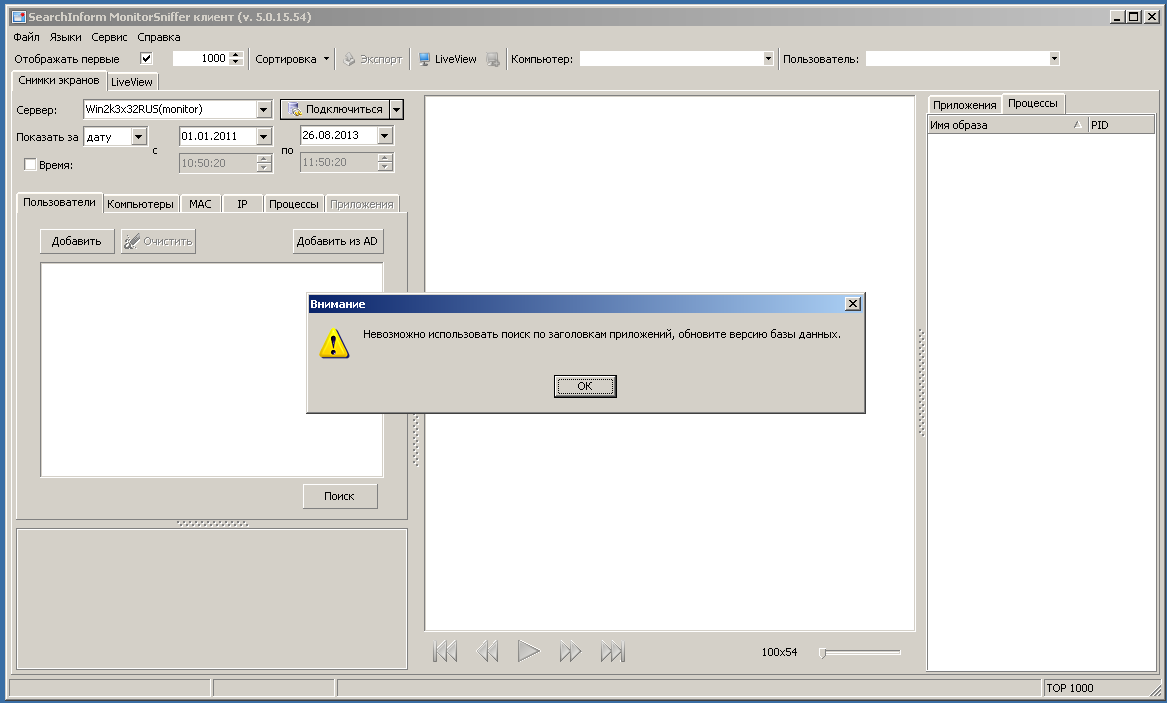
\includegraphics[width=\textwidth]{part2/5}
\end{figure}

\begin{figure}[H]
  \centering
  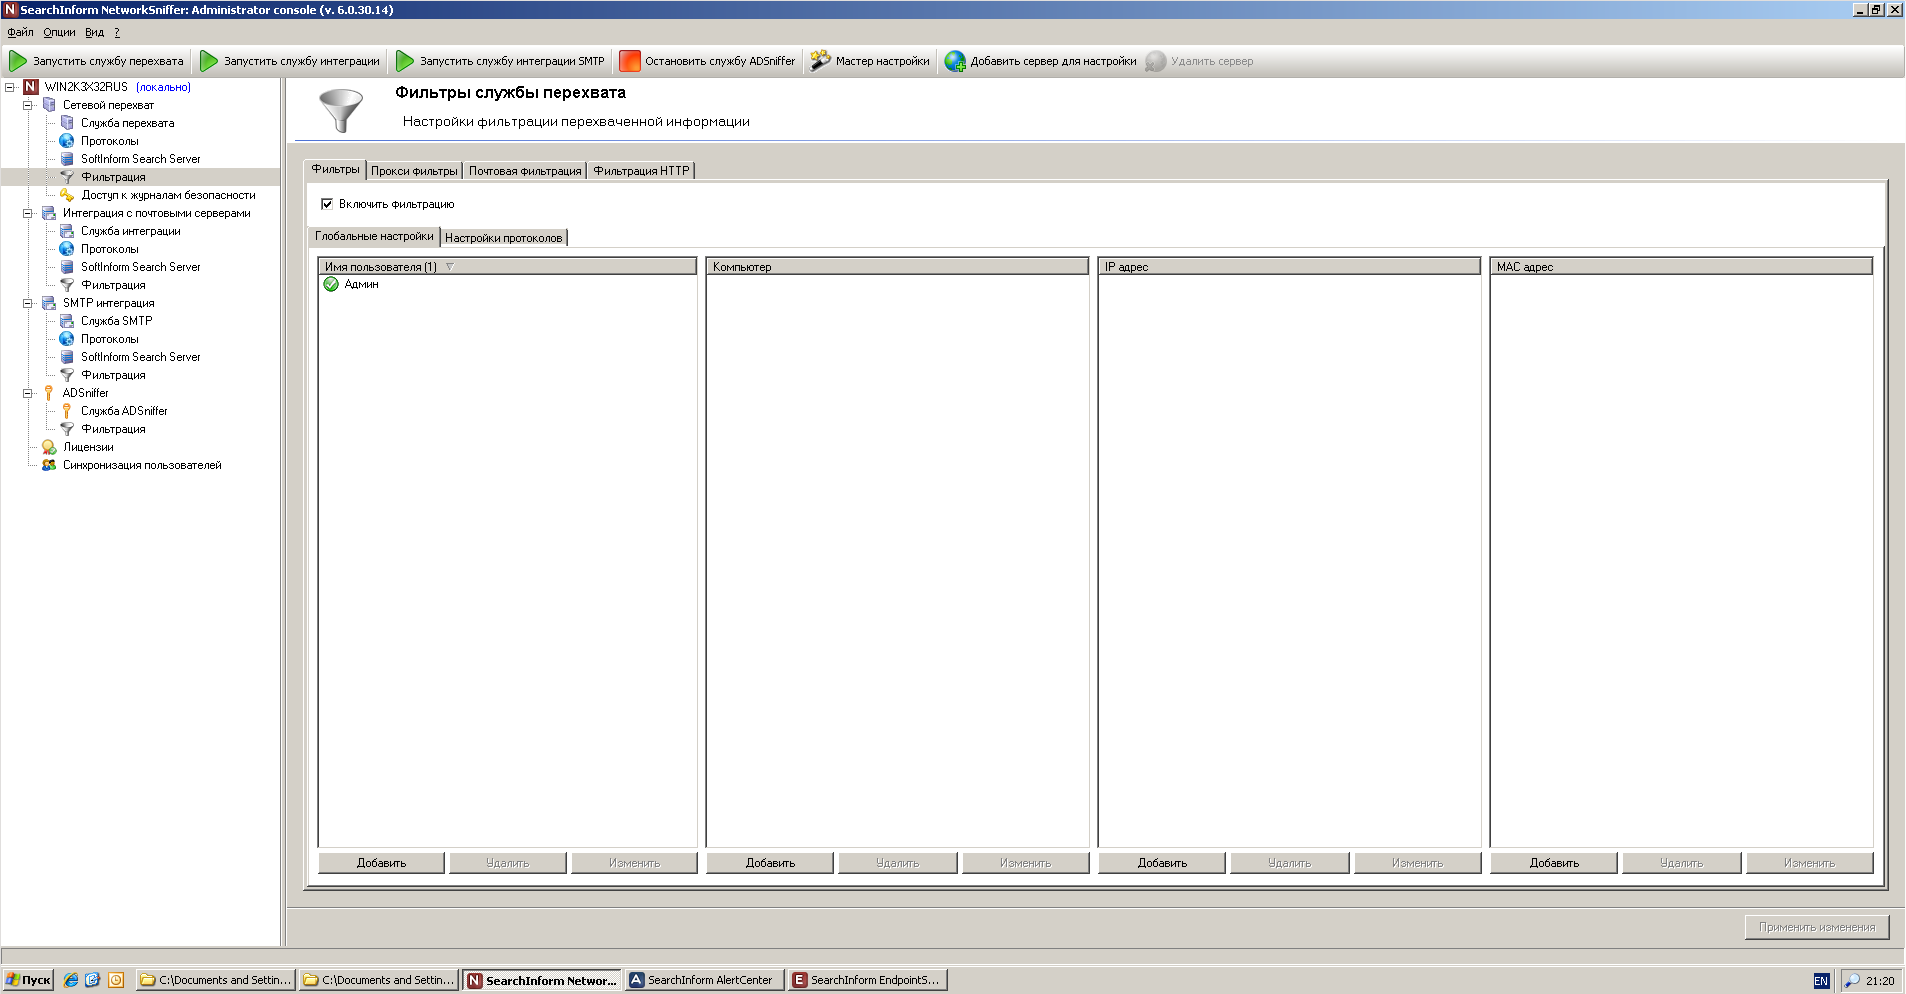
\includegraphics[width=\textwidth]{part2/6}
\end{figure}

\begin{figure}[H]
  \centering
  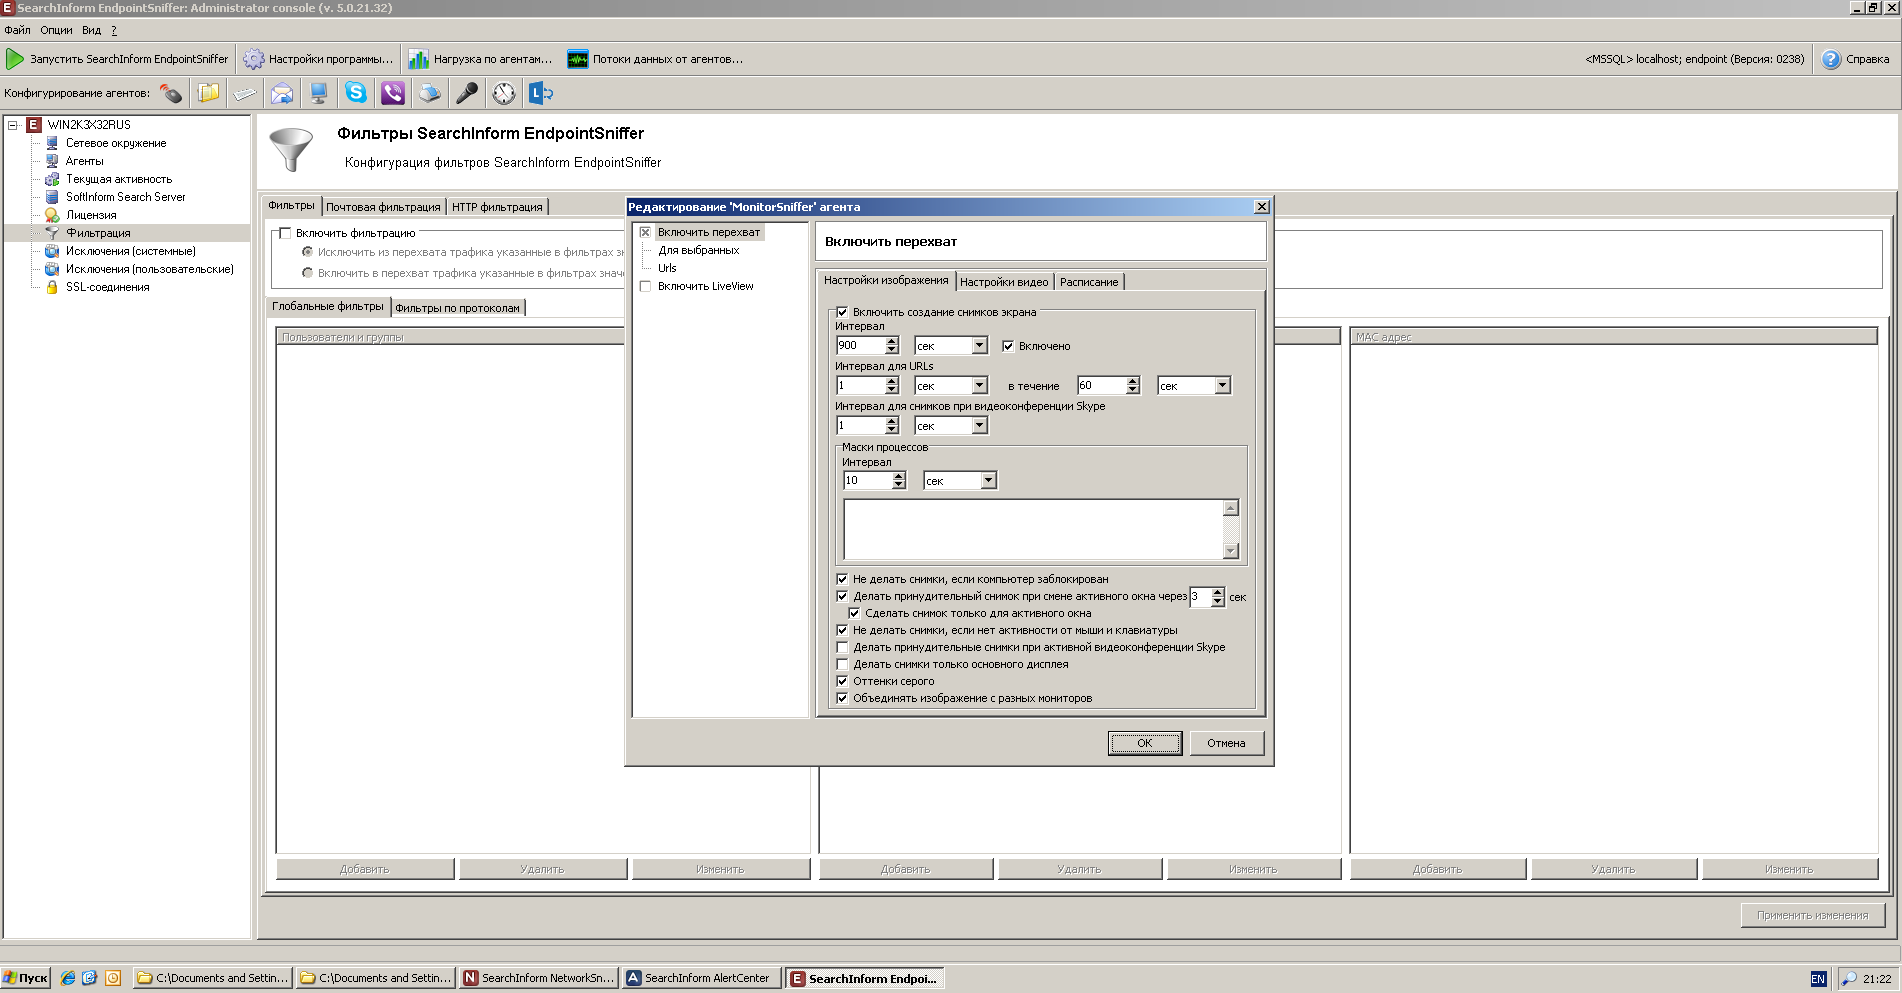
\includegraphics[width=\textwidth]{part2/7}
\end{figure}

\begin{figure}[H]
  \centering
  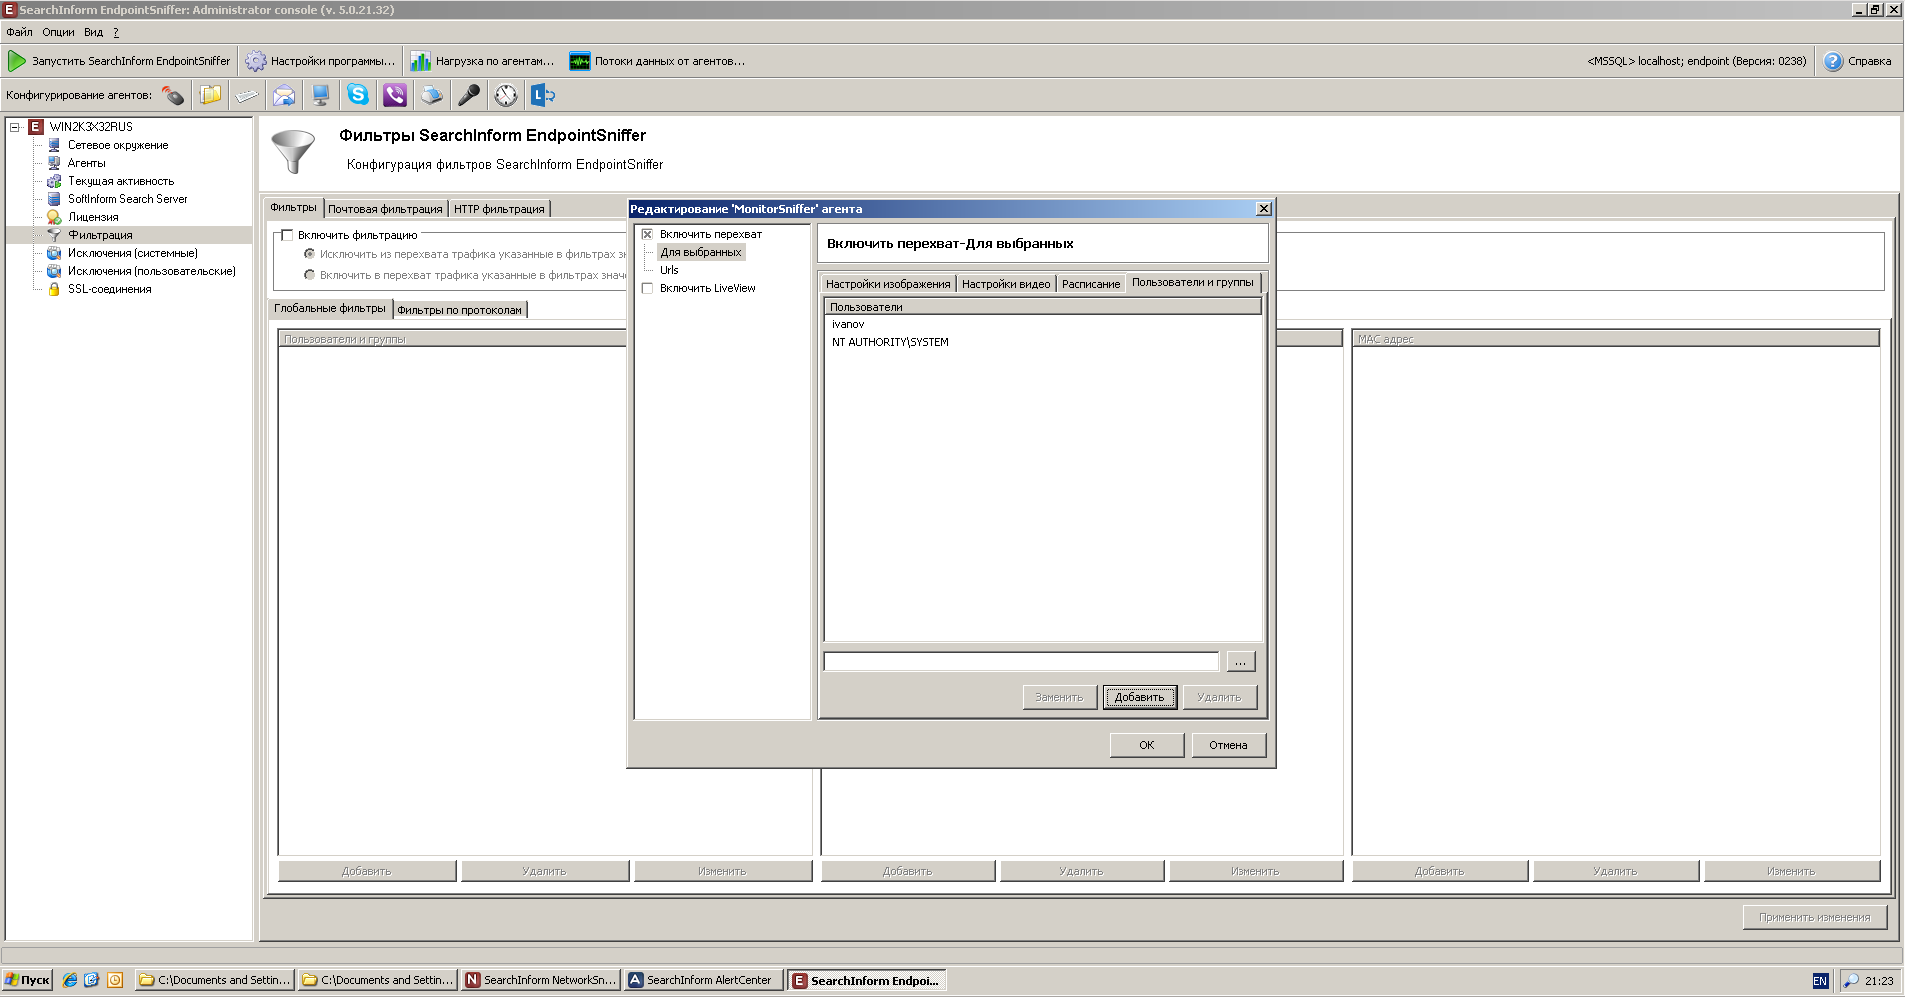
\includegraphics[width=\textwidth]{part2/8}
\end{figure}

\begin{figure}[H]
  \centering
  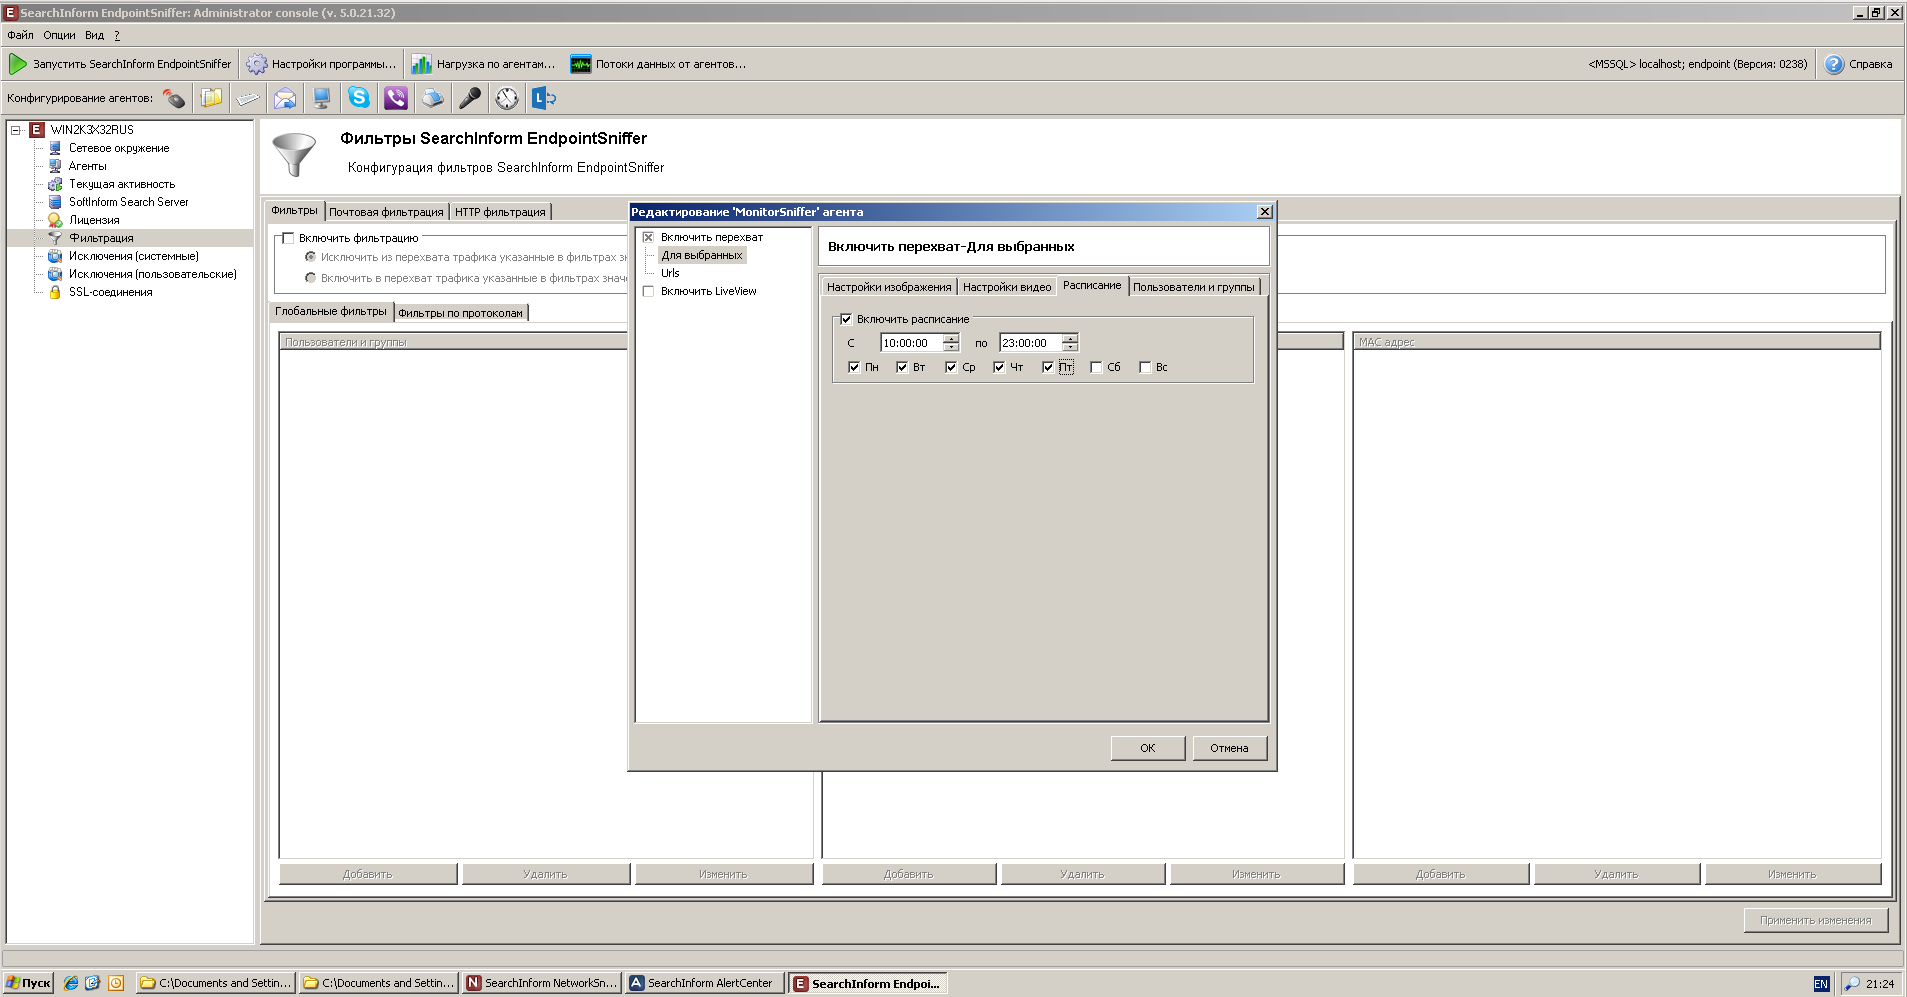
\includegraphics[width=\textwidth]{part2/9}
\end{figure}

\begin{figure}[H]
  \centering
  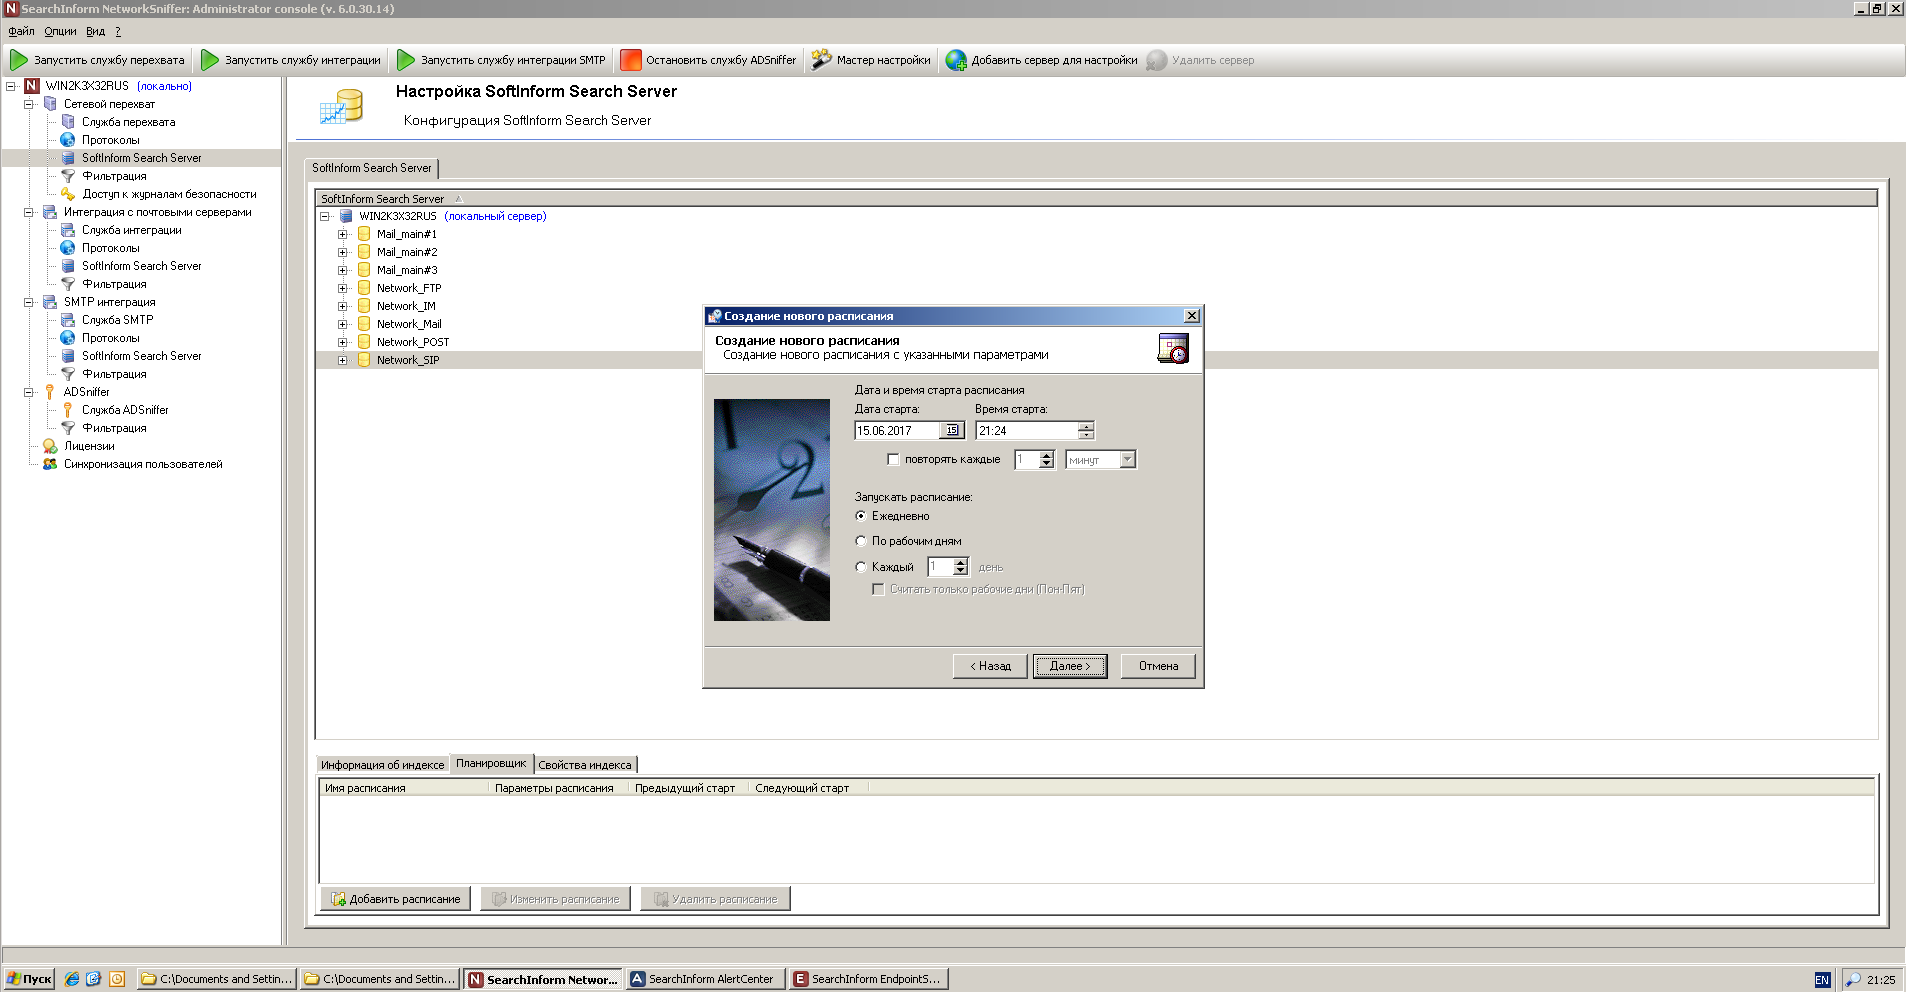
\includegraphics[width=\textwidth]{part2/10}
\end{figure}

\begin{figure}[H]
  \centering
  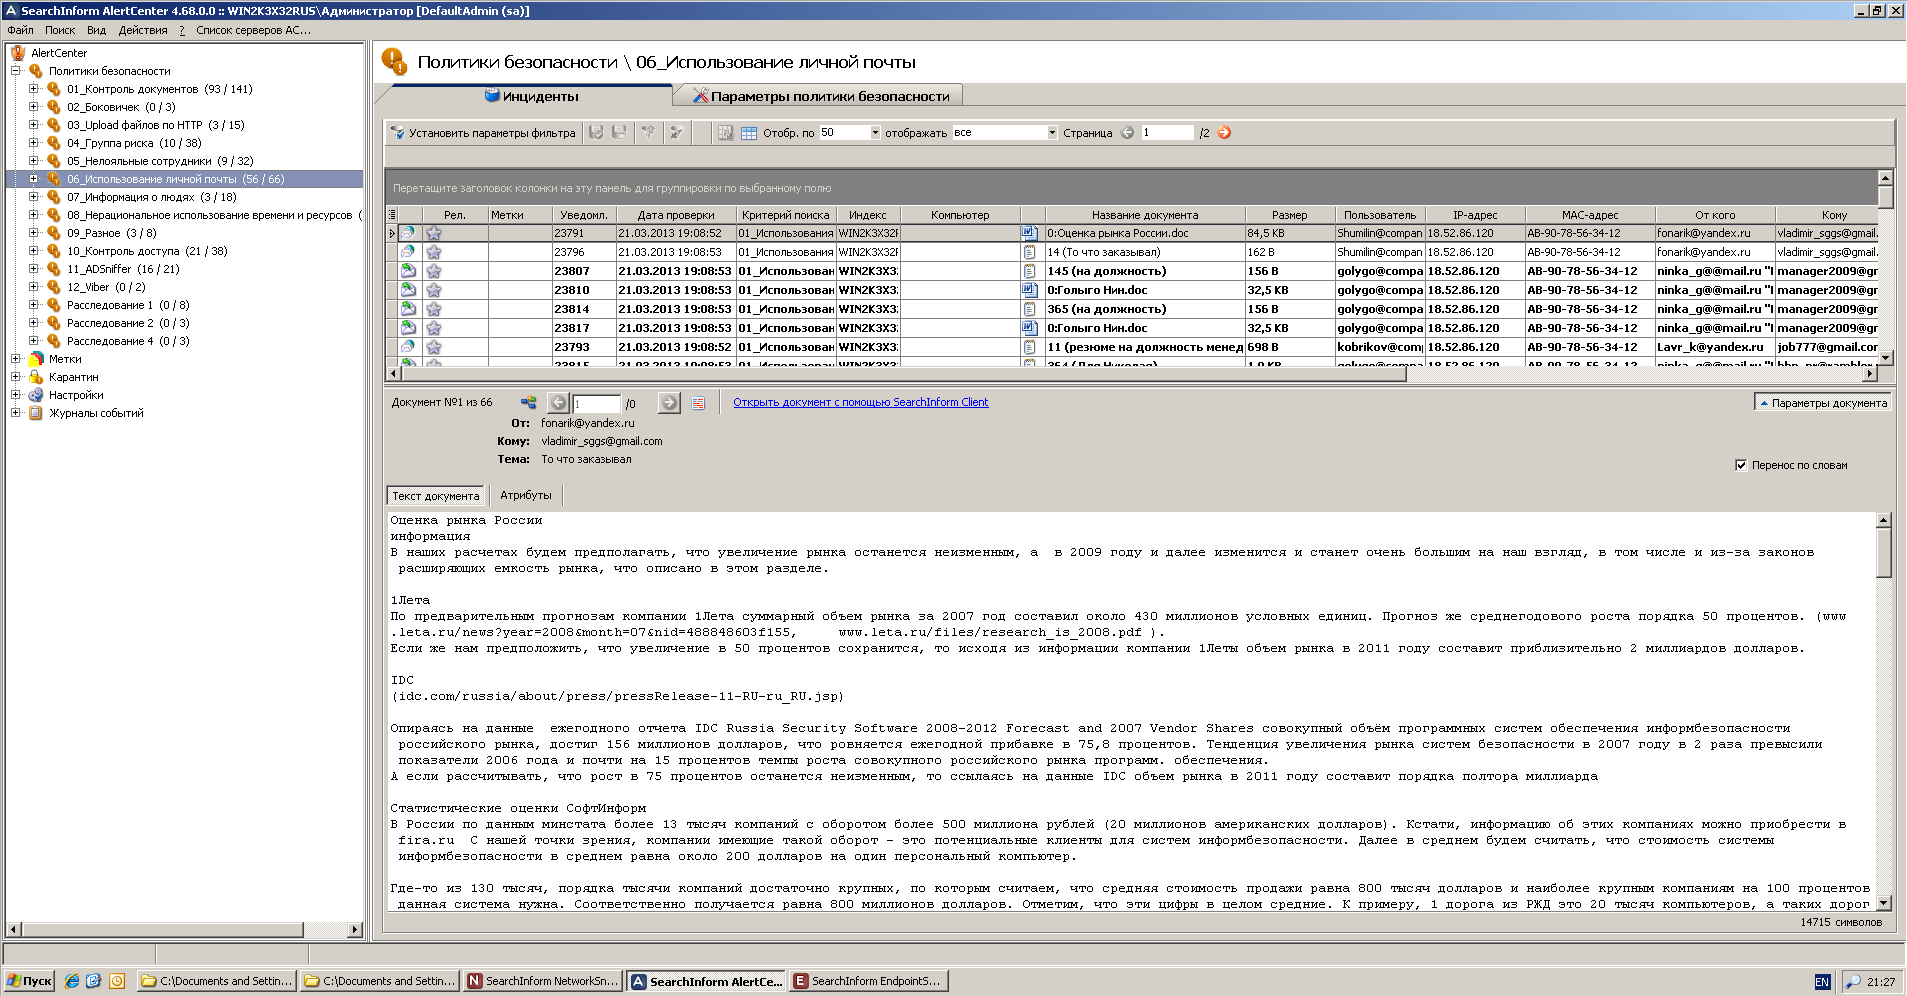
\includegraphics[width=\textwidth]{part2/11}
\end{figure}

\subsection{Контрольные вопросы}

\begin{itemize}
  \item Зачем нужна фильтрация по прокси-серверам?

    Для фильтрации трафика, направленного через конкретный прокси сервер.

  \item Зачем нужна фильтрация по почтовым серверам?

    Для фильтрации писем отправленных пользователями с конкретных почтовых
    серверов.

  \item Какие виды поиска рекомендуются для структурированных документов?

    Поиск по индексам.

  \item Какие виды поиска рекомендуются для не структурированных документов?

    Полнотекстовый поиск.

  \item Что такое «белый список»?

    Фильтр описывающий список разрешенных значений каких-либо атрибутов.

  \item Как используется «разрешающий белый список»?

    Перечисляются значения, которые должны пройти фильтрацию.

  \item Как используется «запрещающий белый список»? 

    Перечисляются значения, которые не должны пройти фильтрацию.

  \item Чем отличается глобальный фильтр от фильтра по протоколам?

    Глобальный фильтр ГЛОБАЛЬНЫЙ, а фильтр по протоколам применяется к
    конкретным протоколам.

  \item Зачем подключать AlertCenter к индексам?

    Для ускорения поиска.

  \item Какой должен быть интервал обновления индексов? 

    Зависит от ситуации.
\end{itemize}
